\section{Introduction}\label{sec:introduction}

Machine learning aims to learn the correct function from data by minimizing the loss between the predicted output and the actual data.
In the process of finding function parameters that will minimize the loss, optimization techniques such as Gradient Descent are utilized.
On the other hand, it is also possible to leverage machine learning techniques in solving optimization problems.
Researchers have conducted numerous studies in this direction~\cite{bengio_machine_2020}.
Particularly, the field of Combinatorial Optimization, which includes NP-hard problems such as the Traveling Salesman Problem and the Knapsack Problem, is one of the playgrounds where machine learning techniques can provide the most significant contributions.

Combinatorial Optimization problems such as the Traveling Salesman Problem, Knapsack Problem, and Set Covering Problem are concerned with finding the optimal solution within the solution set that contains combinations of decision variables’ values.
It is possible to encounter Combinatorial Optimization problems in various fields such as production, logistics, supply chain, and finance.
As the number of decision variables in Combinatorial Optimization problems increases, the number of combinations and the solution time of the optimization problem increase very rapidly.
Therefore, many Combinatorial Optimization problems are NP-hard.
However, the operations research community has developed efficient algorithms that can be used to solve Combinatorial Optimization problems.
The most famous of these algorithms, and the one preferred by commercial optimization software such as CPLEX, is Branch \& Bound~\cite{wolsey_integer_1999}.

Branch \& Bound is an algorithm developed to solve problems that can be formulated as Mixed Integer Programming (MIP) problems, such as Combinatorial Optimization problems.
Branch \& Bound essentially focuses on iteratively dividing the problem into smaller problems (branching) and solving these smaller problems to determine upper and lower bounds on the optimal value of the main problem (bounding).
When upper and lower bounds are equal or when there is no non-investigated node, the optimal value of the problem is reached, and the best feasible solution is the optimal solution.
The choice of the variable to be used for branching in the Branch \& Bound algorithm is one of the most important factors affecting the length of the search tree generated by the algorithm and its performance.
For example, the preference of naive strategies such as most infeasible branching (this branching strategy chooses the variable with the fractional part closest to 0.5) during the selection of the branching variable can reduce the performance of the algorithm by up to 8 times compared to modern branching strategies~\cite{achterberg_mixed_2013}.
Therefore, many researchers have focused on developing strategies for selecting better branching variables in the Branch \& Bound algorithm.
Some of these strategies include Pseudo-cost branching~\cite{benichou_experiments_1971}, Reliability Branching~\cite{achterbergBranchingRulesRevisited2005}, Backdoor Branching~\cite{fischettiBackdoorBranching2011}, Information-based Branching~\cite{kilinckarzanInformationbasedBranchingSchemes2009}, and Strong Branching[7].
Among these strategies, the one that keeps the search tree generated by the algorithm the shortest is Strong Branching [8].
Strong Branching selects the variable that will provide the greatest improvement in the dual bound as the branching variable by trying each potential branching variable one by one at each branching moment.
This strategy keeps the length of the search tree short, but this method is time-consuming as it tries each candidate variable one by one.
Due to its time cost, Strong Branching is impractical in practice.
A study has shown that although the Strong Branching strategy produces on average 65\% fewer search tree nodes compared to the Hybrid Branching strategy preferred by the CPLEX software, it takes 44\% longer on average [8].

\subsection{How to cite a paper}\label{subsec:how-to-cite-a-paper}
This is an example on how to cite a paper~\cite{Tartarini2020a}.

\subsection{How to add acronyms/nomenclature}\label{subsec:how-to-add-acronyms}
This is an example on how to add acronyms.
You can reference the acronym using the command \verb!\ac{t-db}! this will result in the following \ac{t-db}.
If you use the command \verb!\ac{t-db}! again, it will result in \ac{t-db}.
You can check the list of acronyms in the \texttt{myacronyms.tex} file.

\subsection{Glossary}\label{subsec:glossary}

This is an example on how to add a glossary.
You can reference the glossary using the command \verb!\gls{7730}! this will result in the following \gls{7730}.
You can check the list of glossary terms in the \texttt{myglossary.tex} file.

\subsection{How to add a table}\label{subsec:how-to-add-a-table}
This is an example on how to add a table.
The table is shown in Table~\ref{tab:example}.

\begin{table}[htb!]
    \centering
    \begin{tabular}{|c|c|}
        \hline
        \textbf{Column 1} & \textbf{Column 2} \\
        \hline
        Row 1 & Value 1 \\
        Row 2 & Value 2 \\
        Row 3 & Value 3 \\
        \hline
    \end{tabular}
    \caption{This is an example table.}
    \label{tab:example}
\end{table}

\subsection{How to add a figure}\label{subsec:how-to-add-a-figure}
This is an example on how to add a figure.
The figure is shown in Figure~\ref{fig:example}.

\begin{figure}[htb!]
    \centering
    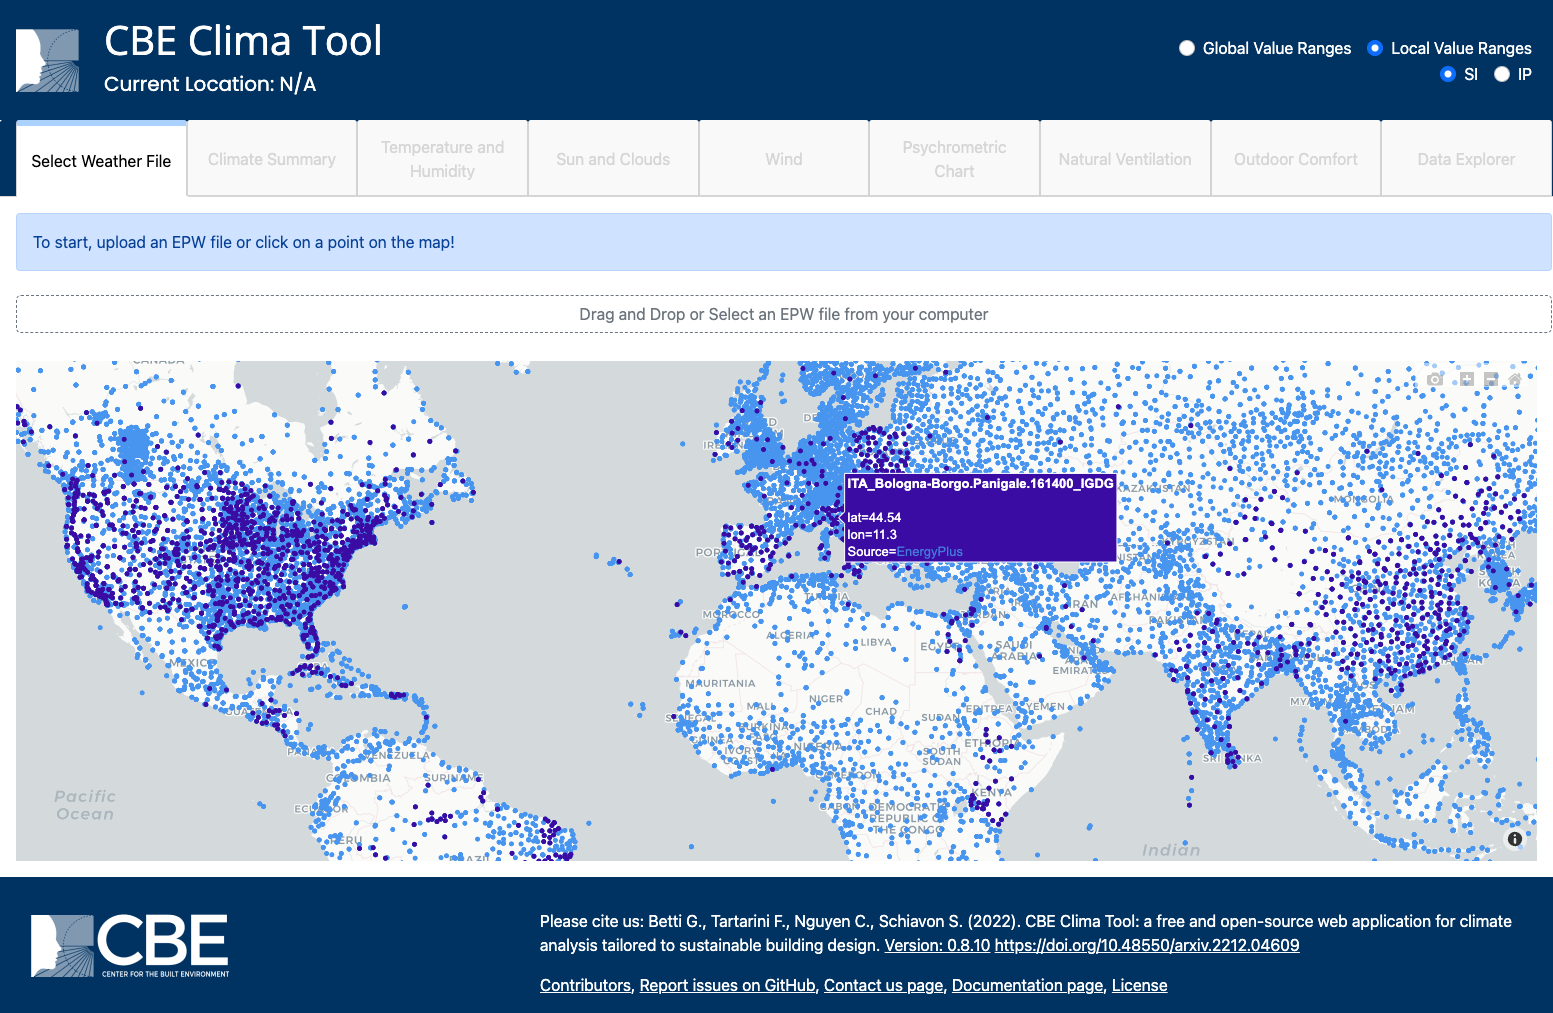
\includegraphics[width=0.75\textwidth]{figures/example_clima}
    \caption{This is an example figure.}
    \label{fig:example}
\end{figure}

\subsection{How to write numbers}\label{subsec:how-to-write-numbers}
This is an example on how to write numbers.

\subsection{How to import a variable}\label{subsec:how-to-import-a-variable}
You can import a variable using the command \verb!\var{example_variable}! this will result in the following \var{example_variable}.
You can check the list of variables in the \texttt{mydata.tex} file.
If you want to find out more on how to import variables, you can check my YouTube video \href{https://ctan.org/pkg/datatool}{datatool} package documentation.